\documentclass{article}

% Importing document settings from our file "packages.sty"
\usepackage{packages}
\pagenumbering{roman} % Start with Roman numerals

% --- Definer forside ---
\title{
    \large INGG2301 -- Ingeniørfaglig systemtenkning \\[0.5em]
    \Large Autonom dronebasert tilstandsovervåking av jernbaneinfrastruktur \\[0.5em]
    \large Prosjektoppgave
}
\author{
    \textbf{Gjøvik 28:} \\
    Elias Fagerbakken Heier \\
    Theodor Sjetnan Utvik \\
    Marcus Minge Wisnes \\
    Halvard Nordberg \\
    Sigurd Riseth
}
\date{\today}

% --- Start dokument ---
\begin{document}

% --- Forside og sammendrag ---
\maketitle
\begin{abstract} % maksimalt 250 ord

\begin{tcolorbox}[
    colback=gray!10,
    colframe=gray!50,
    title=Sammendrag (maksimalt 250 ord) – krav fra oppgaveteksten
]
En kort oppsummering av prosjektrapporten.

\begin{itemize}
    \item Relevans: Hvorfor er det viktig å se nærmere på det dere skriver om i rapporten?
    \item Kort om det underliggende problemet/behovet dere har valgt å ta utgangspunkt i, og hvordan deres konsept (produkt/tjeneste) kan løse dette problemet?
    \item Sammendraget skal inneholde en kort oppsummering av hovedfunn, og overordnet evalueringen av konseptet fra bærekraftsmessig, samfunnsmessig og økonomisk ståsted.
\end{itemize}
\end{tcolorbox}


\end{abstract}

% https://www.sintef.no/en/digital/master-students/automated-drone-based-inspection-of-infrastructure/


\newpage

% --- Innholdsfortegnelse, figurliste, og tabelliste ---
\tableofcontents
\newpage

\listoffigures
\newpage

\listoftables
\newpage

\pagenumbering{arabic}   % Switch to Arabic numerals (1, 2, 3, ...)
\setcounter{page}{1}     % Start page numbering from 1

% --- Hovedinnhold med importerte seksjoner ---
\section{Problembeskrivelse}

\begin{tcolorbox}[
    colback=gray!10,
    colframe=gray!50,
    title=Problem/behov – krav fra oppgaveteksten
]
\textbf{Problem/behov}
\begin{itemize}
    \item Definer og beskriv problemet dere ønsker å løse. Hvem har problemet?
    Hvordan løses dette i dag? Hva er samfunnsmessige ringvirkninger av problemet?
    Hvor stort er problemet (f.eks.\ kan man si noe om hvor mange det berører)?
    Består problemet av flere delproblem?
    \item Basert på informasjon dere henter inn, lag et konsept for en teknologisk
    løsning som har et kommersielt potensial. Løsningen skal henge sammen med
    problemet dere tar utgangspunkt i. Løsningen trenger ikke å beskrives i detalj,
    men jo mer informasjon man har på plass jo enklere vil det være å gjøre
    beregninger senere.
    \item Vurder om problemet er økende sett i lys av samfunnsmessige og
    bærekraftsmessige utfordringer frem mot år 2030. Kan man si at konseptet deres
    støtter nødvendig omstilling for å løse disse utfordringene?
    \item Beskriv styrkene i gruppa som gjør dere godt egnet til å løse dette
    problemet og til å utvikle konseptet.
\end{itemize}
\end{tcolorbox}

\subsection{Problem og behov}

Norges jernbaneinfrastruktur er under betydelig press. Det norske jernbanenettet omfatter om lag 4\,000 kilometer bane, over 2\,700 broer samt et stort antall tunneler og fjellskjæringer \parencite{jernbanedirektoratet_tall}. Mange av disse konstruksjonene er av høy alder og utsatt for kontinuerlig slitasje fra klima, frost og geologiske bevegelser. Det akkumulerte vedlikeholdsetterslepet er estimert til 127,8 milliarder kroner \parencite{banenor_infrastatus_2024}, og til tross for at 437 milliarder kroner er avsatt til jernbaneformål i Nasjonal transportplan (NTP) 2025--2036, vurderer bransjeaktører at dette ikke er tilstrekkelig til å ta inn etterslepet i planperioden \parencite{jernbanedirektoratet_ntp_2025}.

Konsekvensene av utilstrekkelig vedlikehold er målbare. Feil på infrastrukturen sto for om lag 24 prosent av forsinkelsestimene og nærmere 44 prosent av innstilte persontog i andre tertial 2024 \parencite{jernbanedirektoratet_gjennomforingsplan_2025}. Sett over hele 2024 var om lag 34 prosent av persontogene forsinket eller innstilt \parencite{vg_tog_2025}, og Bane NORs punktlighetsmål på 90 prosent ble ikke nådd \parencite{banenor_punktlighet_2025}. Dette rammer arbeidspendlere, reisende og godstransport, og svekker tilliten til jernbanen som foretrukket transportmiddel.

\textit{Primærkundene} -- de som eier problemet -- er infrastrukturforvaltere med ansvar for drift og vedlikehold av jernbanen, i Norge særlig Bane NOR SF. Sekundært berøres togoperatørene (Vy, SJ, GoAhead m.fl.), som er avhengige av infrastrukturens tilstand for å levere punktlige avganger, og i siste instans passasjerene og samfunnet for øvrig.

\subsubsection{Dagens praksis og dens begrensninger}

Bane NOR opererer med to parallelle inspeksjonsspor for jernbanebroer: årlige driftskontroller med begrenset dokumentasjonskrav og grundige ingeniørkontroller hvert sjette år (\cref{kontakt:traetten}). Menneskebetjente droner brukes allerede til bildedokumentasjon ved ingeniørkontroller av broer og høye fjellskjæringer, men krever at en operatør transporteres til stedet for hver gjennomgang (\cref{kontakt:traetten}). For spormåling benyttes i tillegg målevognen Roger 1000 (\cref{kontakt:lau}). Den største operative utfordringen er sportilgang: strenge sikkerhetsregler krever togfrie perioder, som presser inspeksjoner til nattarbeid og begrenser hva som faktisk gjennomføres innenfor et år (\cref{kontakt:traetten}). Den viktigste svakheten i dagens regime er imidlertid ikke datainnsamlingen, men dataanalysen -- innsamlede data sammenlignes fortsatt i stor grad manuelt mot grenseverdier, uten systematisk utnyttelse av historiske trender (\cref{kontakt:lau}).

Problemet kan dekomponeres i tre delproblem:

\begin{enumerate}
    \item \textbf{Lav inspeksjonsfrekvens.} Inspeksjonsintervallet er fast, ikke tilstandsbasert, slik at tilstandsforringelse som oppstår mellom planlagte gjennomganger kan forbli uoppdaget. Eldre infrastruktur kan feile uten forvarsel (\cref{kontakt:traetten}).
    \item \textbf{Personellrisiko.} Manuell inspeksjon i og nær spor og på høye broer medfører HMS-risiko. Krav til sikkerhetsvakter begrenser i tillegg effektiv utnyttelse av tilgjengelig inspeksjonstid (\cref{kontakt:traetten}).
    \item \textbf{Reaktivt vedlikehold.} Mangel på kontinuerlige tilstandsdata og automatisert analyse gjør det vanskelig å drive prediktivt vedlikehold. AI-drevet analyse trekkes frem som det største enkeltforbedringspotesialet i dagens inspeksjonsregime (\cref{kontakt:lau}).
\end{enumerate}

\subsection{Teknologisk konsept}

Konseptet tar utgangspunkt i et konkret og dokumentert markedsbehov (\textit{market pull}), men muliggjøres av kommersielt tilgjengelig droneteknologi og moden AI-basert bildeanalyse som nå er klar for industriell anvendelse (\textit{technology push}). Kombinasjonen av disse to kreftene skaper et gunstig mulighetsvindu \parencite{torvatn_teknologiledelse_2024}.

Det foreslåtte konseptet er et autonomt dronesystem for kontinuerlig tilstandsovervåking av kritiske infrastrukturobjekter langs jernbanen -- tunneler, broer og fjellskjæringer. Systemet består av autonome droner stasjonert i dedikerte dokkingstasjoner plassert permanent ved utvalgte objekter. Dronene utfører forhåndsdefinerte eller hendelsesstyrte inspeksjonsruter -- for eksempel etter kraftig nedbør, frostperioder eller registrerte trafikkavvik -- og samler inn bilde- og sensordata som analyseres over tid for å avdekke gradvise endringer i konstruksjonenes tilstand. En konseptuell illustrasjon av systemet i operasjon er vist i \cref{fig:drone_concept}, mens den overordnede systemarkitekturen er vist i \cref{fig:system_overview}.

\begin{figure}[ht]
    \centering
    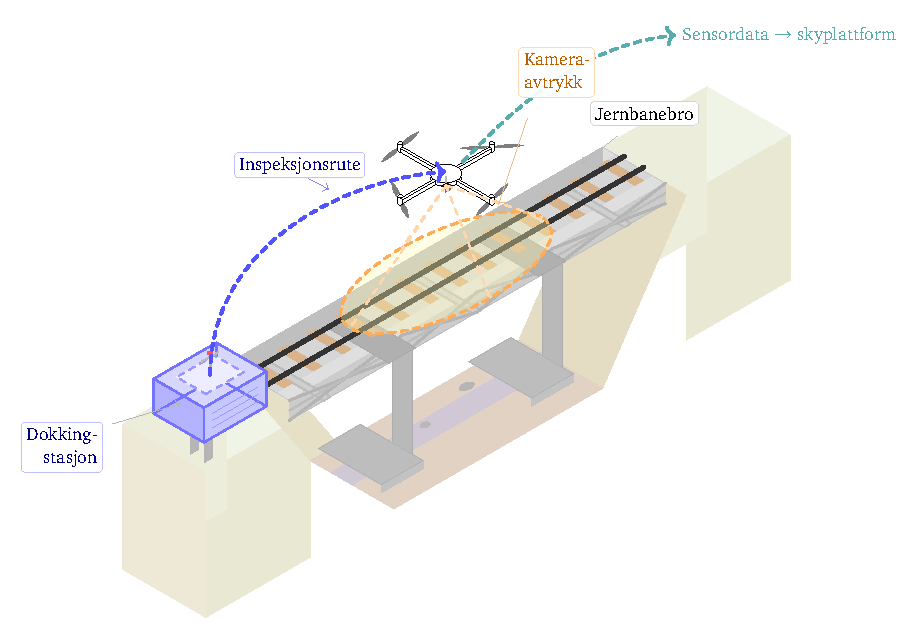
\includegraphics[width=\textwidth]{figurer/drone_figure.pdf}
    \caption{Konseptuell illustrasjon av det autonome dronesystemet i operasjon over en jernbanebro. Dronen letter fra sin permanente dokkingstasjon, følger en forhåndsdefinert inspeksjonsrute og samler inn bilde- og sensordata (oransje kameraavtrykk) som overføres til en skyplattform for analyse.}
    \label{fig:drone_concept}
\end{figure}

\begin{figure}[ht]
    \centering
    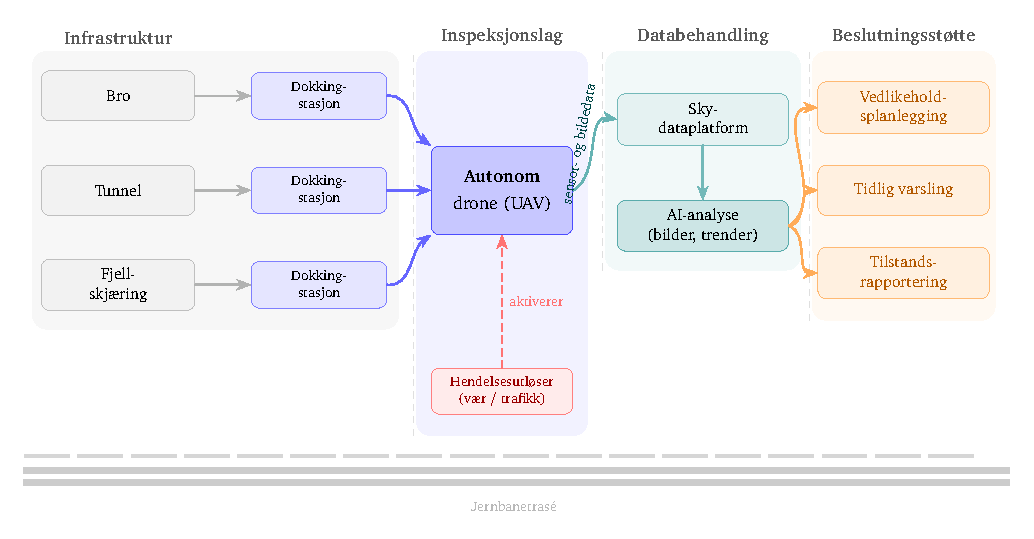
\includegraphics[width=\textwidth]{figurer/system_overview.pdf}
    \caption{Overordnet systemarkitektur. Broer, tunneler og fjellskjæringer utstyres med permanente dokkingstasjoner hvorfra autonome droner utfører planlagte eller hendelsesstyrte inspeksjoner. Innsamlede data overføres til en skybasert plattform for AI-analyse og genererer beslutningsstøtte i form av vedlikeholdsplanlegging, tidlig varsling og tilstandsrapportering.}
    \label{fig:system_overview}
\end{figure}

Konseptet har tydelige paralleller til pågående initiativ internasjonalt. I Spania har luftfartsmyndigheten AESA gitt selskapet Ineco tillatelse til å benytte autonome droner i dokkingstasjoner til jernbaneinspeksjon \parencite{railwaygazette_spain_2024}. Den internasjonale jernbaneunionen (UIC) driver prosjektet Drone4Rail, som i samarbeid med EASA utvikler et regulatorisk rammeverk for langdistanse BVLOS-inspeksjon av jernbane \parencite{uic_drone4rail_2024}. EU-prosjektet RADIUS (Railway Digitalisation Using Drones) har videre utarbeidet konsepter for droneintegrerte dokkingstasjoner og trafikkstyring \parencite{euspa_radius_2024}. I Norden gjennomførte EU-prosjektet Drones4Safety verdens første vellykkede landing og lading av en autonom drone på en høyspentlinje, demonstrert ved Aarhus Letbane i 2022. Prosjektet estimerer et besparelsespotensial på €15 mrd. årlig for europeisk transportinfrastruktur ved full kommersialisering (\cref{kontakt:ebeid}).

Også i Norge er behovet empirisk bekreftet. Bane NOR omtaler automatisert tilstandsovervåking internt som «vegen videre for jernbanen», og et konkret prosjekt med autonom dronestasjon på Meråkerbanen i Trøndelag er planlagt igangsatt 2026--2027 med midler allerede bevilget (\cref{kontakt:traetten}). Nordic Unmanned, en norsk droneoperatør, drifter allerede syv permanente drone-i-boks-systemer for kritisk infrastruktur i Belgia og Finnmark og gjennomførte om lag 2\,500 flyvninger i 2025 (\cref{kontakt:wike}). Disse initiativene bekrefter at det teknologiske og regulatoriske grunnlaget for konseptet er i ferd med å modnes, og at norsk jernbane er godt posisjonert for tidlig adopsjon.

Innovasjonsmessig er konseptet primært en \textit{inkrementell innovasjon}: droner og jernbaneinspeksjon eksisterer begge som separate fenomener, og løsningen kombinerer disse på en ny måte. Konseptet har likevel et element av \textit{disruptiv innovasjon} ved at det retter seg mot et kundesegment -- behovet for kontinuerlig, hendelsesstyrt tilstandsovervåking -- som dagens aktører ikke betjener \parencite[]{torvatn_teknologiledelse_2024}.

Konseptets verdiforslag kan formuleres slik: [PRODUKTNAVN] hjelper infrastrukturforvaltere som Bane NOR, som i dag mangler kontinuerlig og kostnadseffektiv tilstandsovervåking av kritiske jernbanestrukturer, til å gå fra reaktivt til prediktivt vedlikehold -- uten at inspeksjonspersonell trenger å oppholde seg i spor eller på høye konstruksjoner.

\subsection{Problemets utvikling mot 2030}

Problemet må vurderes som \textit{voksende} frem mot 2030, av tre grunner. For det første eldes jernbaneinfrastrukturen raskere enn den fornyes, slik at vedlikeholdsetterslepet øker år for år. For det andre er klimaendringene forventet å øke hyppigheten av ekstreme værhendelser som kraftig nedbør, flom og ras -- hendelser som direkte truer jernbaneinfrastruktur og øker behovet for hyppig tilstandsovervåking. For det tredje skaper den politiske satsingen på jernbane som ryggraden i et bærekraftig transportsystem -- slik det fremgår av NTP 2025--2036 \parencite{jernbanedirektoratet_ntp_2025} -- et økt behov for pålitelig og kostnadseffektiv forvaltning av eksisterende infrastruktur. Den dypere bærekraftsmessige analysen av konseptet, herunder livsløpsvurdering og kobling til FNs bærekraftsmål, behandles i \cref{sec:miljoanalyse}.

\subsection{Gruppens styrker og kompetanse}

Prosjektgruppen består av fem tredjårsstudenter i ingeniørutdanning ved NTNU: to med fordypning i elektroingeniørfag og tre i dataingeniørfag. Den tverrfaglige sammensetningen dekker sentrale deler av det foreslåtte systemet -- sensorteknologi og signalbehandling på den ene siden, og programmering, maskinlæring, datalagring og systemutvikling på den andre -- og gir gruppen et solid teknisk grunnlag for å analysere og videreutvikle konseptet.

Gjennom faglige og personlige nettverk har gruppen tilgang til kontakter med erfaring fra kollektivtransport og jernbanerelatert virksomhet, blant annet fra Sporveien og NTNU-miljøet rundt jernbane og autonome systemer. Dette åpner for kvalitative intervjuer med fagpersoner som besitter innsikt i operative utfordringer, sikkerhetskrav og praktiske rammebetingelser for inspeksjon og vedlikehold -- noe som vil styrke det empiriske grunnlaget for prosjektet.

Gruppen er bevisst på at videre kommersialisering vil kreve kompetanse som gruppen foreløpig ikke besitter: primært innen flysertifisering og BVLOS-regulering, jernbanespesifikke HMS-krav og kommersiell anskaffelsesprosess mot offentlig sektor. For å dekke disse kompetansegapene vil gruppen arbeide systematisk med å identifisere samarbeidspartnere, herunder norske droneselskaper med erfaring fra BVLOS-operasjoner, juridiske rådgivere innen luftfartsrett og eventuelle industripartnere med erfaring fra Bane NOR-prosjekter. En slik partnerstruktur er i tråd med anbefalinger fra faglitteraturen om at teknologioppstartsselskaper bør kompensere for manglende bransjekunnskap gjennom strategiske allianser \parencite[84]{torvatn_teknologiledelse_2024}.

\subsection{Grunnhypoteser}

I tråd med \textcite[57]{torvatn_teknologiledelse_2024} etableres følgende
grunnhypoteser som utgangspunkt for mulighetsstudiet:

\begin{enumerate}
    \item \textbf{Problem--løsning.} Produktet/tjenesten løser problemet med manglende kontinuerlig, kostnadseffektiv og sikker tilstandsovervåking av kritisk jernbaneinfrastruktur ved å tilby autonome, permanent stasjonerte droneinstallasjoner som utfører hendelsesstyrte inspeksjoner uten direkte menneskelig involvering.

    \item \textbf{Kunde.} Primærkunden er infrastrukturforvaltere med ansvar for drift og vedlikehold av jernbane -- i første omgang Bane NOR SF i det norske markedet, med potensial for skalering til øvrige europeiske jernbaneforvaltere.

    \item \textbf{Betalingsvilje.} Kunden vil kjøpe løsningen fordi den reduserer kostnader knyttet til reaktivt vedlikehold og driftsavbrudd, forbedrer HMS for inspeksjonspersonell og gir et bedre og mer kontinuerlig beslutningsgrunnlag for prioritering av vedlikeholdstiltak. Betalingsvilje er empirisk bekreftet: Bane NOR har allerede bevilget midler til et droneovervåkingsprosjekt på Meråkerbanen (\cref{kontakt:traetten}), og ifølge Albert Lau ved NTNU er slik vilje til stede i bransjen, men forutsetter dokumentert effekt -- gjerne med referanser fra andre europeiske land (\cref{kontakt:lau}).

    \item \textbf{Differensiering.} Løsningen skiller seg fra dagens operatørstyrte droner ved å være permanent stasjonert ved spesifikke kritiske objekter og ved å kombinere hendelsesstyrt inspeksjon med longitudinell dataanalyse. Dette muliggjør tidlig varsling og prediktivt vedlikehold -- noe dagens periodiske, transportbaserte inspeksjonsmetoder ikke kan tilby.

    \item \textbf{Markedsvindu.} Det er en unik mulighet i markedet fordi jernbanesektoren globalt er midt i en digitaliseringsbølge, det europeiske regulatoriske rammeverket for BVLOS-operasjoner er i ferd med å modnes, og norsk jernbane har et akutt og erkjent behov for mer effektiv infrastrukturforvaltning -- kombinert med politisk prioritering av vedlikehold i NTP 2025--2036. Ifølge Albert Lau ved NTNU er de organisatoriske og regulatoriske barrierene større enn de tekniske (\cref{kontakt:lau}), noe som gir et fortrinn for aktører som posisjonerer seg tidlig i samarbeid med Bane NOR.
\end{enumerate}

Som et innledende rammeverk for de videre analysene presenteres i \cref{tab:pestel} en PESTEL-analyse av konseptet.

\begin{table}[ht]
    \centering
    \begin{tabular}{p{2cm}p{5cm}p{5cm}}
        \toprule
        \textbf{Forhold} & \textbf{Positive faktorer} & \textbf{Negative faktorer} \\
        \midrule
        Politiske &
        NTP 2025--2036 prioriterer vedlikehold og fornying av jernbane;
        regjeringens satsing på digitalisering og grønn transport &
        Offentlige anskaffelsesprosesser er langsomme og ressurskrevende;
        regulatorisk kompleksitet knyttet til BVLOS-godkjenning fra
        Luftfartstilsynet \\
        \addlinespace
        Økonomiske &
        Vedlikeholdsetterslep på 127,8 mrd.\ kr skaper stort marked;
        dronemarkedet for jernbaneinspeksjon vokser med 24\,\% CAGR mot
        2030; tjenestemodell (drone-as-a-service) senker terskelen for
        kundene &
        Høye initielle investeringskostnader for utvikling og installasjon;
        budsjettkutt i offentlig sektor kan forsinke anskaffelser \\
        \addlinespace
        Sosiale &
        Økt sikkerhet for inspeksjonspersonell ved å redusere arbeid i og
        nær spor; bedre regularitet styrker tilliten til jernbanen som
        samferdselsmiddel &
        Potensiell motstand mot automatisering fra fagforeninger og
        eksisterende inspeksjonspersonell \\
        \addlinespace
        Teknologiske &
        Moden og kommersielt tilgjengelig droneteknologi; fremskritt innen
        AI-basert bildeanalyse og BVLOS-kommunikasjon; EU-prosjekter
        (RADIUS, Drone4Rail) bygger regulatorisk og teknisk grunnlag &
        Krav om høy driftspålitelighet i krevende nordiske klimaforhold
        (kulde, fukt, is); begrenset batterilevetid; utfordringer med
        GPS-ytelse i og rundt tunneler \\
        \addlinespace
        Miljømessige &
        Erstatter fossildrevne inspeksjonskjøretøy;
        muliggjør tilstandsbasert vedlikehold som reduserer overforbruk
        av materialer; støtter klimatilpasning av infrastruktur &
        Produksjon og avfallshåndtering av litium-batterier og
        dronekomponenter har et miljøfotavtrykk \\
        \addlinespace
        Legale &
        EASA-harmonisering av droneregler i Europa åpner for skalering
        på tvers av landegrenser; standardscenarier (STS) forenkler
        driftsgodkjenning for kvalifiserte operatører &
        BVLOS-operasjoner krever individuell driftstillatelse fra
        Luftfartstilsynet med SORA-risikovurdering; usikkerhet rundt
        ansvar ved uønskede hendelser med autonome systemer \\
        \bottomrule
    \end{tabular}
    \caption{PESTEL-analyse for konseptet med autonome dronesystemer til
    jernbaneinspeksjon.}
    \label{tab:pestel}
\end{table}
\section{Mulighetsanalyse}

\subsection{Markedspotensial}

Primærkunden, den som eier problemet og har budsjettansvar, er Bane NOR SF. Brukerne er bane- og bruingeniører samt vedlikeholdspersonell som konsumerer tilstandsdata som grunnlag for prioritering og utbedring. I dag dekkes behovet gjennom årlige driftskontroller og ingeniørkontroller hvert sjette år, supplert med operatørstyrte droner og målevognen Roger~1000 (\cref{kontakt:traetten}). Ekstern inspeksjonskapasitet kjøpes fra aktører som Axess Group og droneoperatører på rammeavtale, men løsningene er arbeidsintensive og gir ikke et kontinuerlig tilstandsbilde (\cref{kontakt:eide}).

Konseptet skaper verdi langs tre akser. Kontinuerlig tilstandsovervåking muliggjør tidligere feildeteksjon og reduserer nedetid ved at begynnende skader fanges opp før de utvikler seg til driftsstans. Løsningen reduserer HMS-kostnader ved å fjerne personell fra spor og høye konstruksjoner, og adresserer samtidig sportilgangsutfordringen der inspeksjoner i dag presses til nattarbeid i togfrie perioder (\cref{kontakt:traetten}). Kontinuerlig dataanalyse gir i tillegg grunnlag for en overgang fra reaktivt til prediktivt vedlikehold.

Markedet segmenteres naturlig etter infrastrukturtype (bro, tunnel, fjellskjæring) og kritikalitet. Vi fokuserer på \emph{punktovervåking av høyrisikolokasjoner} fremfor flåtedekning, ettersom dagens dronebokser har begrenset rekkevidde og er lite egnet til lineær inspeksjon over lange strekninger (\cref{kontakt:wike}). Primærsegmentet er skred- og rasutsatte punkter, som Trætten fremhever som det mest prekære overvåkingsbehovet i Bane NOR og hvor det allerede er bevilget midler til en autonom dronestasjon på Meråkerbanen (\cref{kontakt:traetten}). Sekundært adresseres de mest kritiske av Bane NORs 2\,700+ broer~\cite{jernbanedirektoratet_tall}, særlig eldre stålbruer, overgangssoner og flomutsatte fundamenter (\cref{kontakt:sjetnan}), der eksakt omfang må kartlegges mot Bane NORs egen klassifisering i konsekvensklasser. Det globale markedet for dronebasert jernbaneinspeksjon er estimert til å vokse fra 1,67~mrd.~USD i 2025 til 4,86~mrd.~USD i 2030, tilsvarende en årlig vekst (CAGR) på om lag 24~\%~\cite{businessresearch_drone_2025}. Veksten drives av lettelser i BVLOS-regelverket, aldrende infrastruktur og modning av AI-drevne plattformer for prediktivt vedlikehold.

Når det gjelder prising, foreslår vi en hybrid modell: salg av dokkingstasjon og drone som engangskostnad på 1--1,5~MNOK per objekt, basert på referansetall fra Nordic Unmanned (\cref{kontakt:wike}), pluss et årlig abonnement på analyseplattform og drift anslått til 200--300~kNOK per objekt. Modellen reflekterer to sammenfallende preferanser: Bane NOR ønsker eierskap til utstyr og data (\cref{kontakt:traetten}), mens droneoperatørene foretrekker forutsigbare inntekter (\cref{kontakt:wike}). Betalingsvilje er empirisk bekreftet gjennom bevilgningen til Meråkerbanen-prosjektet. Samtidig illustrerer Nordic Unmanneds fireårige rammeavtale fra 2021, der forventet omsetning på 30~MNOK endte på om lag 436\,000~kr før selskapet gikk konkurs i februar 2025~\cite{aga_forventet_2025, dahl_droneselskap_2025}, at nominelle rammeavtaler med Bane NOR ikke automatisk konverterer til reell omsetning. Realistisk prising må derfor ta høyde for lav faktisk utnyttelse og lang ledetid fra signert avtale til fakturert aktivitet.


\subsection{Forretningsmodell, kommersialisering og økonomiske betraktninger}

\subsubsection{Forretningsmodellen}
\label{sec:forretningsmodell}

Kundesegmentet består primært av jernbaneinfrastrukturforvaltere med BaneNOR som første målgruppe. Verdien skapes gjennom økt inspeksjonsfrekvens, bedre beslutningsgrunnlag og redusert nedetid. Inntektsmodellen kan enten være en tjenestemodell (drone-as-a-service) eller en hybrid modell hvor kunden eier systemet og betaler for drift og analyse. Sistnevnte støttes av bransjeinnsikt som viser at kunder ofte ønsker eierskap til data og utstyr. Nøkkelressurser inkluderer dronebaser, AI-basert analyse og regulatorisk kompetanse, mens nøkkelpartnere vil være droneselskaper, teknologileverandører og juridiske aktører innen luftfartsregelverk.

\begin{figure}[ht]
    \centering
    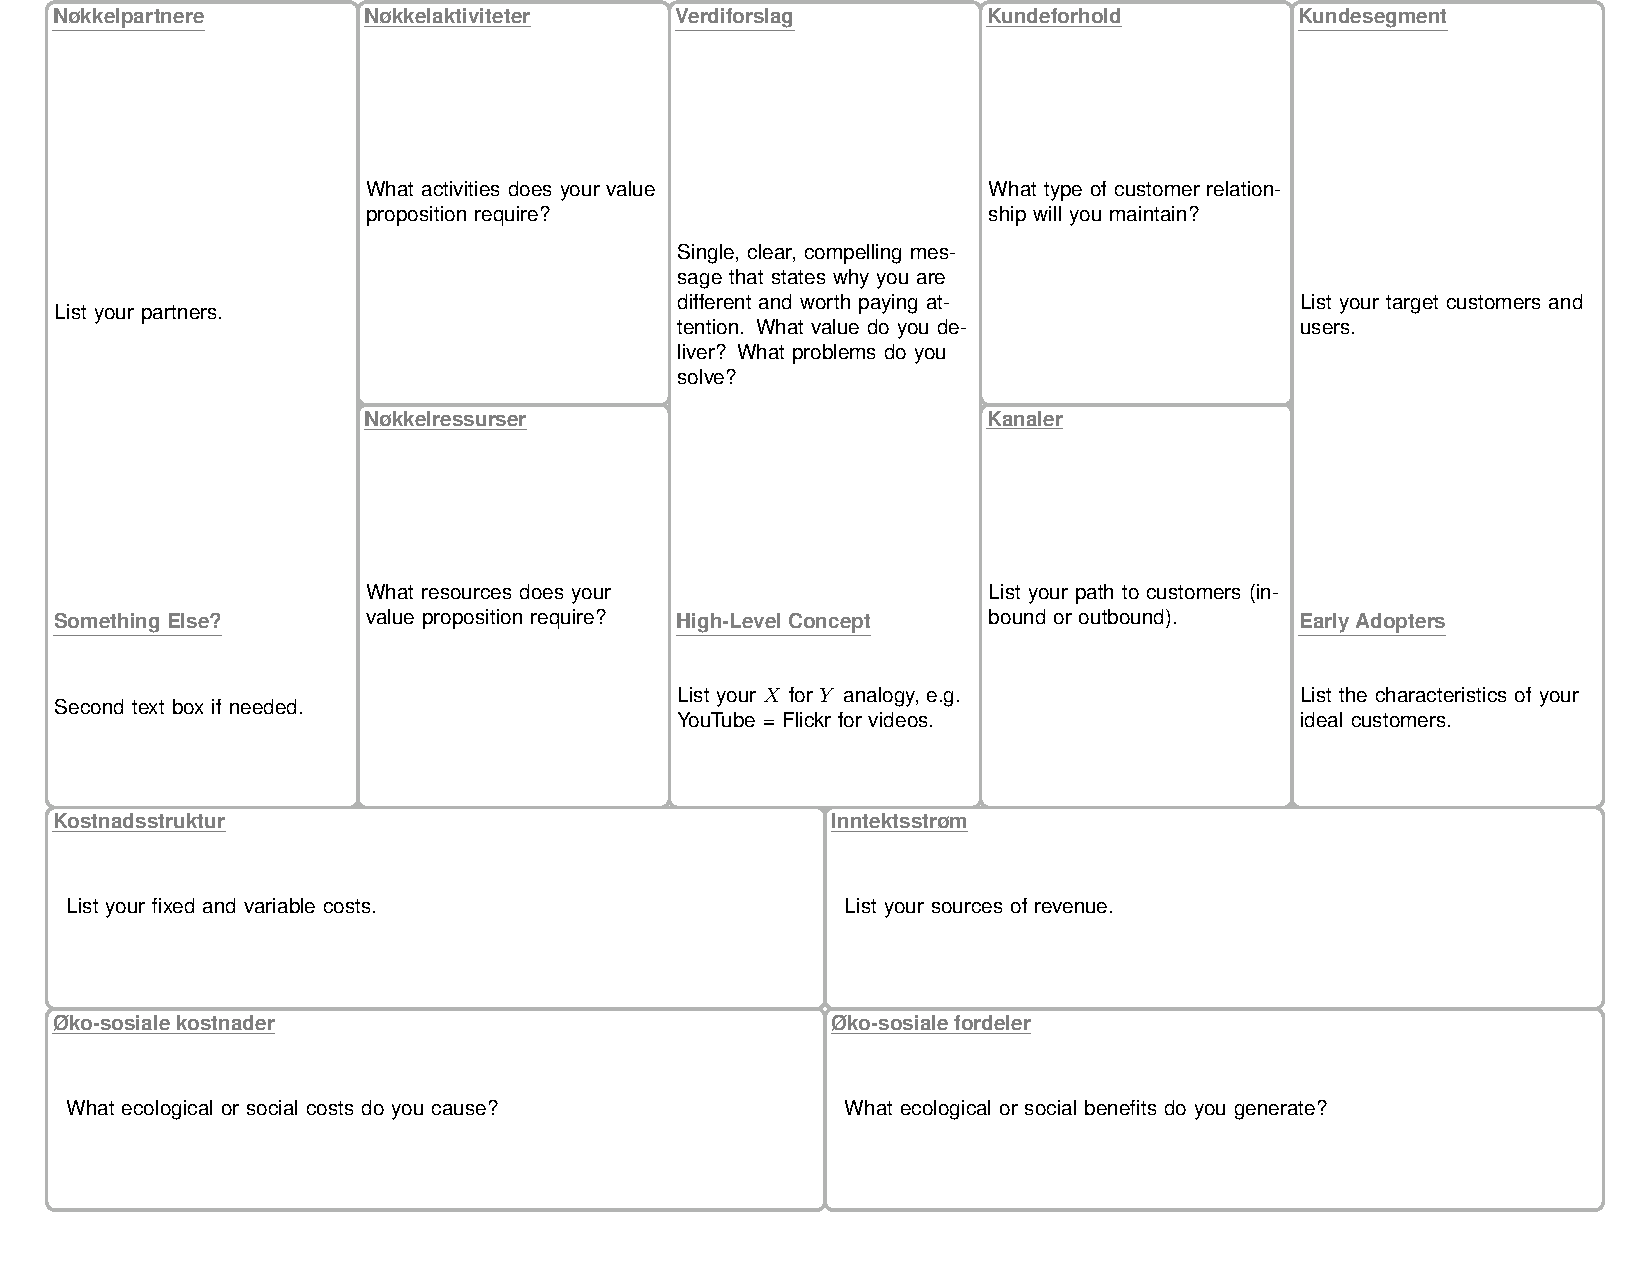
\includegraphics[width=1.0\linewidth]{figurer/Lerret_for_forretningsmodell.pdf}
    \caption{Utvidet \textit{Business Model Canvas} (lerret for forretningsmodell).}
    \label{fig:lerret-for-forretningsmodell}
\end{figure}

\subsubsection{Kommersialisering}
Kommersialiseringen vil skje stegvis, med pilotprosjekter ved utvalgte kritiske infrastrukturobjekter for å dokumentere effekt og redusere risiko. Dette er i tråd med eksisterende initiativer i bransjen hvor implementering av ny teknologi skjer gradvis og krever dokumentert nytteverdi. Videre skalering vil skje gjennom langsiktige kontrakter med infrastrukturforvaltere. Eventuelt i samarbeid med etablerte droneoperatører. Viktige barrierer inkluderer regulatoriske krav, særlig knyttet til BVLOS-operasjoner samt komplekse offentlige anskaffelsesprosesser. Konseptet befinner seg i en tidlig fase med høyt kapitalbehov og usikkerhet, men også et betydelig markedspotensial drevet av økende behov for effektiv og sikker infrastrukturforvaltning.

\subsubsection{Økonomiske betraktninger: kostnader, inntekter og finansiering}
\label{sec:okonomi}

Vår virksomhet kan klassifiseres som en vekstbedrift i idé- og utviklingsfasen, kjennetegnet av intensiv FoU, høy usikkerhet, betydelig kapitalbehov og omfattende ulønnet egeninnsats fra grunderne \parencite{torvatn_teknologiledelse_2024}. Det
økonomiske oppsettet består derfor av et drifts-, investerings- og likviditetsbudsjett for 2027, strukturert etter Altinns veileder for oppstartsbedrifter \parencite{altinn_budsjett} og retningslinjene i INGG2301. De fullstendige budsjettene er presentert i \cref{app:driftsbudsjett}.

Fem grundere tar delvis lønn på ca.\ 15\,000~NOK brutto per måned (20\,000~NOK inkl.\ sosiale kostnader per person, totalt 100\,000~NOK/mnd), mens resterende arbeidsinnsats er ulønnet egeninnsats. Investeringene på ca.\ 1,48~MNOK omfatter én prototypedrone (DJI~Matrice~350~RTK med Zenmuse~P1-payload), AI-utviklingsarbeidsstasjoner, testrigg og programvarelisenser, avskrevet lineært over fem år. Dokkingstasjoner og pilotinstallasjon utsettes til etablerings- og kommersialiseringsfasen i år 2--3. Samlede driftskostnader beløper seg til ca.\ 1,8~MNOK.

Utviklingsåret budsjetteres tilnærmet inntektsløst, slik læreboken beskriver som typisk for første driftsår i FoU-tunge virksomheter \parencite{torvatn_teknologiledelse_2024}. Vi budsjetterer kun 75\,000~NOK fra sporadiske konsulent- og rådgivningsoppdrag. Den hybride salgs- og abonnementsmodellen beskrevet i \cref{sec:forretningsmodell} aktiveres først ved pilotavtale i år~2.

Kapitalbehovet på ca.\ 3,3~MNOK dekkes av egenkapital, soft funding og kassakreditt. Tilskuddsbasert finansiering ble valgt fremfor aksjeemisjon for å bevare grundernes eierandeler og som ekstern kvalitetsvurdering av teknologien. Break-even-analysen indikerer at 2--3 dokkingstasjoner i stabil drift er tilstrekkelig for lønnsomhet.

Timingen er like kritisk som summen. SkatteFUNN-refusjonen på 500\,000~NOK inngår i finansieringsplanen, men utbetales først via skatteoppgjøret i år~2 og bidrar med null kroner til kontantstrømmen i 2027. Dette skaper et strukturelt underskudd gjennom hele året som forsterkes av CAPEX-tyngdepunktet i januar–mars. Likviditetsbudsjettet viser et maksimalt kassakredittbehov på ca.\ 1,57~MNOK i desember, som overstiger rammen på 1,3~MNOK med om lag 270\,000~NOK. Gapet kan lukkes gjennom leasing av drone, utsatt anskaffelse eller en fremskyndet utbetalingsprofil med Innovasjon Norge.
\section{Miljøanalyse og bærekraftperspektiver}
\label{sec:miljoanalyse}

\begin{tcolorbox}[colback=gray!10, colframe=gray!50, title=Miljøanalyse og bærekraftperspektiver - Krav fra oppgaveteksten]

Analyser den miljømessige og sosiale/samfunnsmessige bærekraften for konseptet. Analysen
skal inneholde følgende:

\begin{itemize}
    \item \textbf{Relasjon til utviklingsmål}. Betrakt norske og/eller internasjonale politiske utviklingsmål for klima, energi, ressursbruk og bærekraftig utvikling som er relevante for deres konsept og vurder hvordan forretningsideen deres vil passe med disse utviklingsmålene. Slike koblinger kan være endret etterspørsel og/eller marked for konfliktbelagte ressurser, andre ressursbegrensninger (energi, materialer, arealer eller annet), tilbakekoblingseffekter eller annet. 
    \item \textbf{Bidrag til bærekraftig utvikling}. Fastsett de viktigste aspektene/faktorene ved problemet og løsningen med tanke på bærekraft. Vurder om det det er aspekter ved produksjon, bruk eller avhending av konseptet (som produkt eller tjeneste) som kan være problematisk eller fordelaktige for energi, klima, ressursbruk, helse, økosystemer eller andre miljøaspekter. Beskriv og begrunn hvordan konseptet kan bidra positivt til bærekraftig utvikling, eller hvordan det kan utformes slik at miljøkonsekvenser minimeres.
    \item \textbf{Miljøanalyse}. Bruk som grunnlag én eller flere av metodene for miljøvurdering som vi beskriver i dette emnet: livsløpsvurdering, fotavtrykksanalyse og materialstrømsanalyse. Dette kan være egne (forenklede) analyser, eller bruk av data fra studier gjort av andre for lignende eller tilknyttede konsept. Velg metoden(e) som per mest relevant(e) for konseptet. Gjør antagelser og begrunn dem det er nødvendig. Om det gjenstår spørsmål som dere ikke kan svare ut, beskriv hvordan dette eventuelt kan gjøres. 
\end{itemize}
\end{tcolorbox}

Dette kapittelet analyserer konseptets miljømessige og samfunnsmessige bærekraft i tre deler: (i) relasjon til overordnede politiske utviklingsmål, (ii) konseptets bidrag til bærekraftig utvikling, og (iii) en forenklet livsløpsvurdering (LCA) som kvantitativt grunnlag for miljøvurderingen. Detaljerte mellomregninger er samlet i \cref{app:beregninger}.

\subsection{Relasjon til utviklingsmål}

Konseptet med autonome droner for jernbaneinspeksjon er tett knyttet til sentrale nasjonale og internasjonale mål innen klima, infrastruktur og bærekraftig transport.

\subsubsection{FNs bærekraftsmål}

Av FNs 17 bærekraftsmål er særlig tre direkte relevante.

\textbf{SDG~9 – Industri, innovasjon og infrastruktur} er det mest sentrale. Delmål~9.1 vektlegger utvikling av robust og bærekraftig infrastruktur, mens delmål~9.4 omhandler økt ressurseffektivitet. Dronesystemet bidrar til begge ved å styrke robustheten gjennom raskere feildeteksjon og muliggjøre mer målrettet, behovsbasert vedlikehold fremfor faste inspeksjonsintervaller.

\textbf{SDG~11 – Bærekraftige byer og lokalsamfunn} er relevant fordi jernbanen er en nøkkelkomponent i et bærekraftig transportsystem. Delmål~11.2 fremhever behovet for trygge og tilgjengelige transportløsninger. Infrastrukturrelaterte avvik utgjorde 24\,\% av forsinkelsestimene i andre tertial 2024 \parencite{jernbanedirektoratet_gjennomforingsplan_2025}, noe som svekker jernbanens konkurranseevne. Konseptet kan redusere slike avvik og dermed styrke jernbanens attraktivitet som transportform.

\textbf{SDG~13 – Stoppe klimaendringene} er relevant både direkte og indirekte. Direkte gjennom reduksjon av utslipp fra inspeksjonsaktivitet, og indirekte gjennom økt klimatilpasningsevne. Delmål~13.1 fremhever robusthet mot klimarelaterte hendelser; her gir kontinuerlig overvåking bedre beslutningsgrunnlag etter ekstremvær.

\subsubsection{Norske klimamål}

Norge har som mål å redusere klimagassutslipp med minst 55\,\% innen 2030 sammenlignet med 1990-nivå \parencite{miljodirektoratet_klimamal}. Transportsektoren er en sentral kilde til utslipp og prioritert for reduksjon. Dagens inspeksjonsmetoder — helikopter og dieselkjøretøy — inngår i disse utslippene. Konseptet erstatter disse med elektriske løsninger basert på fornybar energi og er dermed godt i tråd med nasjonale prioriteringer. Videre understøtter konseptet klimatilpasning ved å muliggjøre rask kartlegging etter ekstremvær.

\subsubsection{EUs grønne vekststrategi}

EUs \textit{European Green Deal} har som mål å redusere transportutslipp med 90\,\% innen 2050 og fremhever digitalisering som et sentralt virkemiddel \parencite{ec_green_deal}. Konseptet adresserer begge dimensjoner ved å redusere fossile utslipp og digitalisere inspeksjonsprosesser. For en løsning med ambisjon om europeisk skalering er denne tilpasningen også strategisk viktig.

\subsection{Bidrag til bærekraftig utvikling}

Basert på etablerte kategorier for miljømessig bærekraft identifiseres tre sentrale dimensjoner: klimagassutslipp og energibruk, materialressurser og avfall og sosiale forhold knyttet til arbeidsliv og sikkerhet.

\subsubsection{Positive aspekter}

\textbf{Reduserte klimagassutslipp.} Den mest direkte gevinsten er substitusjon av fossilbasert inspeksjon med elektriske droner. Med norsk strømmiks, som har svært lavt karbonfotavtrykk (23\,g~\ce{CO2eq}/kWh \parencite{nve_kraftproduksjon}), blir driftsutslippene minimale sammenlignet med helikopter- og dieselbaserte alternativer.

\textbf{Mer ressurseffektivt vedlikehold.} Kontinuerlig tilstandsdata muliggjør prediktivt vedlikehold, som reduserer behovet for akutte og ressursintensive reparasjoner. Dette kan gi betydelige indirekte miljøgevinster, selv om disse er vanskelige å kvantifisere uten tilgang til vedlikeholdshistorikk fra Bane NOR.

\textbf{Forbedret HMS.} Bruk av droner reduserer behovet for arbeid i risikofylte omgivelser — nær spor eller i høyden — og bidrar dermed positivt til sosial bærekraft.

\subsubsection{Negative aspekter og avbøtende tiltak}

\textbf{Batteriproduksjon og råmaterialer.} Produksjon av litium-ion-batterier er forbundet med betydelige utslipp og utfordringer knyttet til utvinning av kritiske materialer som kobolt og litium. Valg av leverandører med dokumentert ansvarlig utvinning og bruk av batterityper med lavere koboltinnhold (f.eks.\ LFP-kjemi) kan redusere denne belastningen.

\textbf{Elektronikkavfall.} Systemet genererer EE-avfall ved endt levetid. Effektiv innsamling og gjenvinning i henhold til EUs WEEE-direktiv er avgjørende for å minimere miljøbelastningen. Produsentansvar bør innarbeides i forretningsmodellen.

\textbf{Energibruk til digital infrastruktur.} Databehandling og lagring krever energi, men effekten kan begrenses ved bruk av datasentre med fornybar energimiks og energieffektive algoritmer for bildeprosessering.

\textbf{Sosiale konsekvenser av automatisering.} Automatisering kan påvirke eksisterende arbeidsroller. Dette bør håndteres proaktivt gjennom kompetanseutvikling og tidlig involvering av ansatte, i dialog med Bane NOR.

\subsection{Miljøanalyse}
\label{subsec:lca}

Miljøpåvirkningen vurderes gjennom en forenklet livsløpsvurdering (LCA). Metoden er valgt fordi konseptet innebærer et fysisk system med tydelige livsløpsfaser der de viktigste miljøbidragene varierer mellom produksjon, drift og avhending. Analysen er ikke fullstendig i henhold til ISO~14040/14044, men gir et beslutningsrelevant estimat basert på tilgjengelige data og eksplisitte antagelser. Samtlige mellomregninger er dokumentert i \cref{app:beregninger}.

\subsubsection{Mål- og omfangsdefinisjon}

\paragraph{Formål.}
Analysen skal vurdere klimagassavtrykket (\ce{CO2eq}) av det autonome dronesystemet sammenlignet med dagens inspeksjonspraksis. Formålet er å belyse om klimagevinsten i driftsfasen oppveier produksjonskostnaden, og å identifisere hvilke livsløpsfaser som er dominerende.

\paragraph{Funksjonell enhet.}
\textit{Kontinuerlig tilstandsovervåking og gjennomføring av behovsstyrte inspeksjoner av ett jernbaneobjekt (én bro) over ett kalenderår.}

Referansesystemets tilsvarende funksjon er: \textit{periodisk manuell- og helikopterbasert inspeksjon av samme bro etter dagens praksis.}

\paragraph{Systemgrense.}
Analysen følger et «vugge til grav»-perspektiv for dronesystemet og dekker tre faser:
\begin{enumerate}
    \item \textbf{Produksjon:} råmaterialutvinning, komponentproduksjon og montering av droner og dokkingstasjon.
    \item \textbf{Drift:} energiforbruk til flygning og lading, batteriutskiftning og vedlikehold.
    \item \textbf{Avhending:} deponering og gjenvinning av batterier og elektronikk.
\end{enumerate}
For referansesystemet inkluderes kun driftsfasen (drivstofforbruk helikopter og kjøretøy). Helikoptre og kjøretøy er allerede i bruk til mange formål, og produksjonsutslippet lar seg ikke allokere til inspeksjonsaktiviteten alene uten ytterligere data. Dette er en konservativ antagelse som noe favoriserer dronesystemet, og er identifisert som en svakhet i analysen.

\paragraph{Nøkkelantagelser.}
En fullstendig liste over antagelser og begrunnelser finnes i \cref{app:beregninger}. De viktigste er:
\begin{itemize}
    \item To droner per objekt (DJI Matrice~300~RTK-klasse, ca.\ 9\,kg inkl.\ batteri, 274\,Wh per batteri); levetid 5 år.
    \item Inspeksjonsfrekvens: 52 flygninger per år (én per uke), à 30\,min og 90\,W effektforbruk.
    \item Norsk strømmiks: 23\,g~\ce{CO2eq}/kWh \parencite{nve_kraftproduksjon}.
    \item Referansesystem: 2 helikopterinspeksjoner + 4 manuelle kjøretøyinspeksjoner per år \parencite{johannesen_bane_2021}.
    \item \ce{CO2eq}-faktor for Li-ion-batteriproduksjon: 80\,kg~\ce{CO2eq}/kWh \parencite{lca_battery_2021}.
\end{itemize}

\subsubsection{Resultater}

De beregnede klimagassutslippene er oppsummert i \cref{tab:lca_resultat}. Fullstendig inventaranalyse og alle mellomregninger er gjengitt i \cref{app:beregninger}.

\begin{table}[ht]
    \centering
    \caption{Estimerte klimagassutslipp per bro per år. Alle tall er avrundede estimater; se \cref{app:beregninger} for mellomregninger.}
    \label{tab:lca_resultat}
    \begin{tabular}{llr}
        \toprule
        \textbf{System} & \textbf{Bidragspost} & \textbf{kg~\ce{CO2eq}/år} \\
        \midrule
        \multirow{6}{*}{Dronesystem}
        & Batteriproduksjon (amortisert over levetid)    & 44 \\
        & Elektronikk og ramme (amortisert)              & 16 \\
        & Dokkingstasjon (amortisert over 10 år)         &  6 \\
        & Batteriutskiftning (1 batteri per 2 år)        & 22 \\
        & Ladeenergi (drift)                             & <1 \\
        \cmidrule{2-3}
        & \textbf{Sum dronesystem}                       & \textbf{$\approx$\,88} \\
        \addlinespace
        \hline
        \multirow{3}{*}{Referansesystem}
        & Helikopter (2 inspeksjoner à 1{,}5 t)          & 432 \\
        & Kjøretøy (4 inspeksjoner à 100 km t/r)         &  68 \\
        \cmidrule{2-3}
        & \textbf{Sum referansesystem}                   & \textbf{$\approx$\,500} \\
        \bottomrule
    \end{tabular}
\end{table}

Beregningen viser at dronesystemet slipper ut anslagsvis \textbf{88\,kg~\ce{CO2eq}} per bro per år, mot referansesystemets \textbf{500\,kg~\ce{CO2eq}} — en reduksjon på om lag \textbf{82\,\%}. Produksjonsfasen dominerer dronesystemets utslipp: over 90\,\% stammer fra batterier, elektronikk og dokkingstasjon, mens driftsutslippene er marginale grunnet Norges rene energimiks. For referansesystemet dominerer drivstofforbruk i driftsfasen. Norges jernbanenett har over 2\,700 broer \parencite{jernbanedirektoratet_tall}; innføres systemet ved 500 kritiske objekter, tilsvarer besparelsen omlag $500 \times 412\,\text{kg} \approx \textbf{206\,\text{t}~\ce{CO2eq}/år}$ i direkte inspeksjonsrelaterte utslipp.

\subsubsection{Tolkning}

\paragraph{Funn.}
Analysen indikerer at dronesystemet har vesentlig lavere klimagassutslipp enn referansesystemet. Klimabelastningen fra produksjonsfasen tilbakebetales raskt gjennom reduserte driftsutslipp. I tillegg kommer potensielt store indirekte gevinster fra prediktivt vedlikehold som reduserer akutte, materialintensive reparasjoner — en effekt som ikke er kvantifisert i denne analysen.

\paragraph{Begrensninger og usikkerhet.}
Resultatene er beheftet med usikkerhet på flere punkter. For det første er produksjonsutslippet for dronene estimert fra generiske LCA-data for tilsvarende utstyrsklasse, ikke fra produsentspesifikke data. For det andre er avhendingsfasen ikke fullt modellert, ettersom gjenvinningsrater for batterier og elektronikk varierer betydelig. For det tredje er referansesystemets produksjonsutslipp utelatt, noe som konservativt favoriserer dronesystemet. Til tross for disse svakhetene vurderes hovedkonklusjonen som robust: forskjellen mellom systemene (82\,\%) er stor nok til å absorbere rimelige feilmarginer. For en mer fullstendig analyse anbefales det å innhente EPD-data (Environmental Product Declaration) fra droneprodusenter og faktisk vedlikeholdsstatistikk fra Bane NOR.
\section{Sammenstilling, refleksjon og diskusjon} % Maksimalt 750 ord

\begin{tcolorbox}[colback=gray!10, colframe=gray!50, title=Krav fra oppgaveteksten]

\textbf{Maksimalt 750 ord!}

\begin{itemize}
    \item Sammenstill og diskuter egenskaper ved konseptet deres for økonomisk, samfunnsmessig og miljømessig bærekraft, og avveininger mellom de ulike bærekraftshensynene. Hva er deres vurdering av bærekraft for konseptet? Klarer dere å oppfylle alle målene for problemstillingen og løse det aktuelle problemet?
    \item Reflekter over usikkerhetsmomenter/begrensninger i arbeidet som er gjort.
    \item Er konseptet verdt å gå videre med? Vil dere som gruppe gå videre med prosjektet?
\end{itemize}
\end{tcolorbox}



% --- Litteraturliste ---
\newpage
\printbibliography[heading = bibintoc, title = Litteraturliste]

% --- Vedlegg ---
\newpage
\appendix
\section{Kontaktlogg}
\label{app:kontaktlogg}

Dette vedlegget inneholder en systematisk oversikt over kvalitative intervjuer og samtaler gjennomført i forbindelse med mulighetsanalysen. Formålet med loggen er å dokumentere innsamlet informasjon på en måte som gjør den lett å tolke og bruke videre i utviklingen av forretningsmodellen.

Kontaktpersonene er organisert i fire kategorier basert på rolle: potensielle kunder, brukere, samarbeidspartnere og eksperter. Denne inndelingen gjør det enklere å analysere innsikter ut fra forskjellige perspektiver og identifisere hvilke behov og utfordringer som er mest relevante for problemstillingen.

Som påpekt av \textcite[57]{torvatn_teknologiledelse_2024}, er aktiv kontakt med relevante aktører – herunder kunder, leverandører, produsenter og distributører – avgjørende for å hente informasjon som støtter utforming av forretningsmodellen. Kontaktloggen følger derfor en struktur som registrerer hver interaksjon, inkludert dato, ansvarlig student og kontaktinformasjon, slik at innsamlet data kan brukes systematisk i analysen.

Ved å dokumentere alle telefonsamtaler, e-poster og møter sikrer loggen at viktig informasjon ikke går tapt. Samtidig gjør den det mulig å tolke og bruke materialet systematisk, slik at både studentgruppen og andre kan dra nytte av innsamlet data i analysen og trekke ut sentrale funn på tvers av kontaktene \parencite[57]{torvatn_teknologiledelse_2024}.

Intervjuene ble gjennomført som semistrukturerte dybdeintervjuer. For hver målgruppe ble det utarbeidet en intervjuguide med faste tema og åpne spørsmål for å sikre både sammenlignbarhet og fleksibilitet. Dette gjorde det mulig å utforske uforutsette innsikter samtidig som sentrale problemstillinger ble dekket i alle samtaler. Samtalene ble dokumentert gjennom notater og oppsummert umiddelbart etter gjennomføring.

\subsection{Kunder}

\subsubsection{Kontakt 1 – Ola Nordmann}

\textbf{Bransje/stilling:} Bla bla bla \\
\textbf{Kontaktinfo:} E-post/tlf/etc. \\
\textbf{Dato:} 12.01.2026 \\
\textbf{Ansvarlig fra studentgruppen:} Én av oss her

\paragraph{Sentrale funn}
Bla bla bla bla...

\subsubsection{Kontakt 2 – Kari Hansen}

\textbf{Bransje/stilling:} \\
\textbf{Kontaktinfo:} \\
\textbf{Dato:} \\
\textbf{Ansvarlig fra studentgruppen:}

\paragraph{Sentrale funn}

\subsection{Brukere}

\subsubsection{Kontakt 3 – Andreas Berg}

\textbf{Bransje/stilling:} \\
\textbf{Kontaktinfo:} \\
\textbf{Dato:}  \\
\textbf{Ansvarlig fra studentgruppen:} 

\paragraph{Sentrale funn}

\subsection{Samarbeidspartnere}

\subsubsection{Kontakt 4 – Ingrid Lunde}

\textbf{Bransje/stilling:}  \\
\textbf{Kontaktinfo:}  \\
\textbf{Dato:} \\
\textbf{Ansvarlig fra studentgruppen:}

\paragraph{Sentrale funn}

\subsection{Eksperter}

\subsubsection{Kontakt 5 – Albert Lau}
\label{kontakt:lau}

\textbf{Fagområde/stilling:} Førsteamenuensis NTNU \\
\textbf{Kontaktinfo:} albert.lau@ntnu.no, +47 942 58 319 \\
\textbf{Dato:} 04.03.2026 \\
\textbf{Ansvarlig fra studentgruppen:} Sigurd Riseth

\paragraph{Sentrale funn} 

Albert Lau bekrefter at jernbaneinfrastruktur er generelt mer sårbar enn veiinfrastruktur, særlig i Norge med mye enkeltspor --- en feil kan stoppe trafikk på hele strekninger. Han trekker frem bruer og sporveksler som de mest kritiske objektene å overvåke, der spesielt sporveksler i trafikkintensive knutepunkter (som Oslo S og Alnabru) har stor operasjonell betydning. Viktigste årsaker til tilstandsforringelse er alder og utmattingsskader (fatigue).

Dagens inspeksjonsmetoder er manuelle inspeksjoner og målevognen Roger 1000. Den største svakheten ligger ikke i datainnsamlingen, men i dataanalysen – data sammenlignes fortsatt i stor grad manuelt mot grenseverdier. Lau peker på AI-drevet analyse som det største forbedringspotensiale, og hans eget forskningsmiljø jobber med nettopp dette.

På spørsmål om barrierer for autonom droneinspeksjon mener han de organisatoriske og regulatoriske utfordringene er større enn de tekniske. Organisatorisk handler det om motstand og skepsis mot ny teknologi. Regulatorisk er datadeling og AI-regulering i Europa særlige utfordringer.

Betalingsvilje for automatiserte overvåkingsløsninger er til stede, men forutsetter dokumentert effekt – gjerne med referanser fra andre europeiske land. Lau nevner at Bane NOR allerede kjøper teknologi fra bl.a. Østerrike, som et eksempel på at slik vilje finnes.

\subsubsection{Kontakt 6 – Emad Samuel Malki Ebeid}

\textbf{Fagområde/stilling:} Professor på Syddansk Universitet, Prosjekt koordinator for Drones4Safety.eu \\
\textbf{Kontaktinfo:} esme@mmmi.sdu.dk \\
\textbf{Dato:} 12.02.2026 \\
\textbf{Ansvarlig fra studentgruppen:} Sigurd Riseth

\paragraph{Sentrale funn} 

Emad bekrefter at Drones4Safety utviklet et system av autonome, selvladende droner for inspeksjon av broer og jernbane. Det mest sentrale resultatet er verdens første vellykkede landing og lading på en høyspentlinje, demonstrert ved Aarhus Letbane i 2022 – noe Emad omtaler som potensielt revolusjonerende for dronebransjen, ettersom typisk flygetid i dag er begrenset til 10–15 minutter.

Prosjektet utviklet sværmalgoritmer for samordnet flerdroneoperasjon, samt AI-algoritmer for automatisk deteksjon av infrastrukturfeil fra dronebilder via skybasert analyse. Systemet ble testet på Asti-broen i Italia og Siemens' jernbanetestsenter i Tyskland.

Emad peker på regulatoriske forhold som den viktigste barrieren for kommersiell utrulling – særlig lovgivning rundt autonom luftfart – og anbefaler å ta tidlig kontakt med relevante myndigheter som EASA og Luftfartstilsynet. Han understreker videre at AI-modeller bør bygge på eksisterende treningsdata fra prosjekter som Drones4Safety fremfor å utvikles fra bunnen av. Han anslår at kommersielt tilgjengelige selvladende droner kan være realitet innen 3–4 år, og estimater indikerer et kostnadsbesparelsespotensial på €15 mrd. årlig for inspeksjon av europeisk transportinfrastruktur.

\subsubsection{Kontakt 7 – Inge Hoff}

\textbf{Fagområde/stilling:} Professor på NTNU \\
\textbf{Kontaktinfo:} inge.hoff@ntnu.no, +47 735 94 731, +47 934 26 463 \\
\textbf{Dato:}  \\
\textbf{Ansvarlig fra studentgruppen:} Sigurd Riseth

\paragraph{Sentrale funn} 

\section{Driftsbudsjett}
\label{app:driftsbudsjett}

Dette vedlegget inneholder det fullstendige økonomiske oppsettet for første driftsår (2027), strukturert etter Altinns veileder for oppstartsbedrifter \parencite{altinn_budsjett}. Budsjettet består av tre deler: et driftsbudsjett med tilhørende break-even-analyse og finansieringsplan, et investeringsbudsjett med månedlige avskrivninger, og et likviditetsbudsjett som viser faktisk kontantstrøm per måned.


% \url{https://info.altinn.no/starte-og-drive/drive-bedrift/okonomi-og-gebyrer/budsjett/}

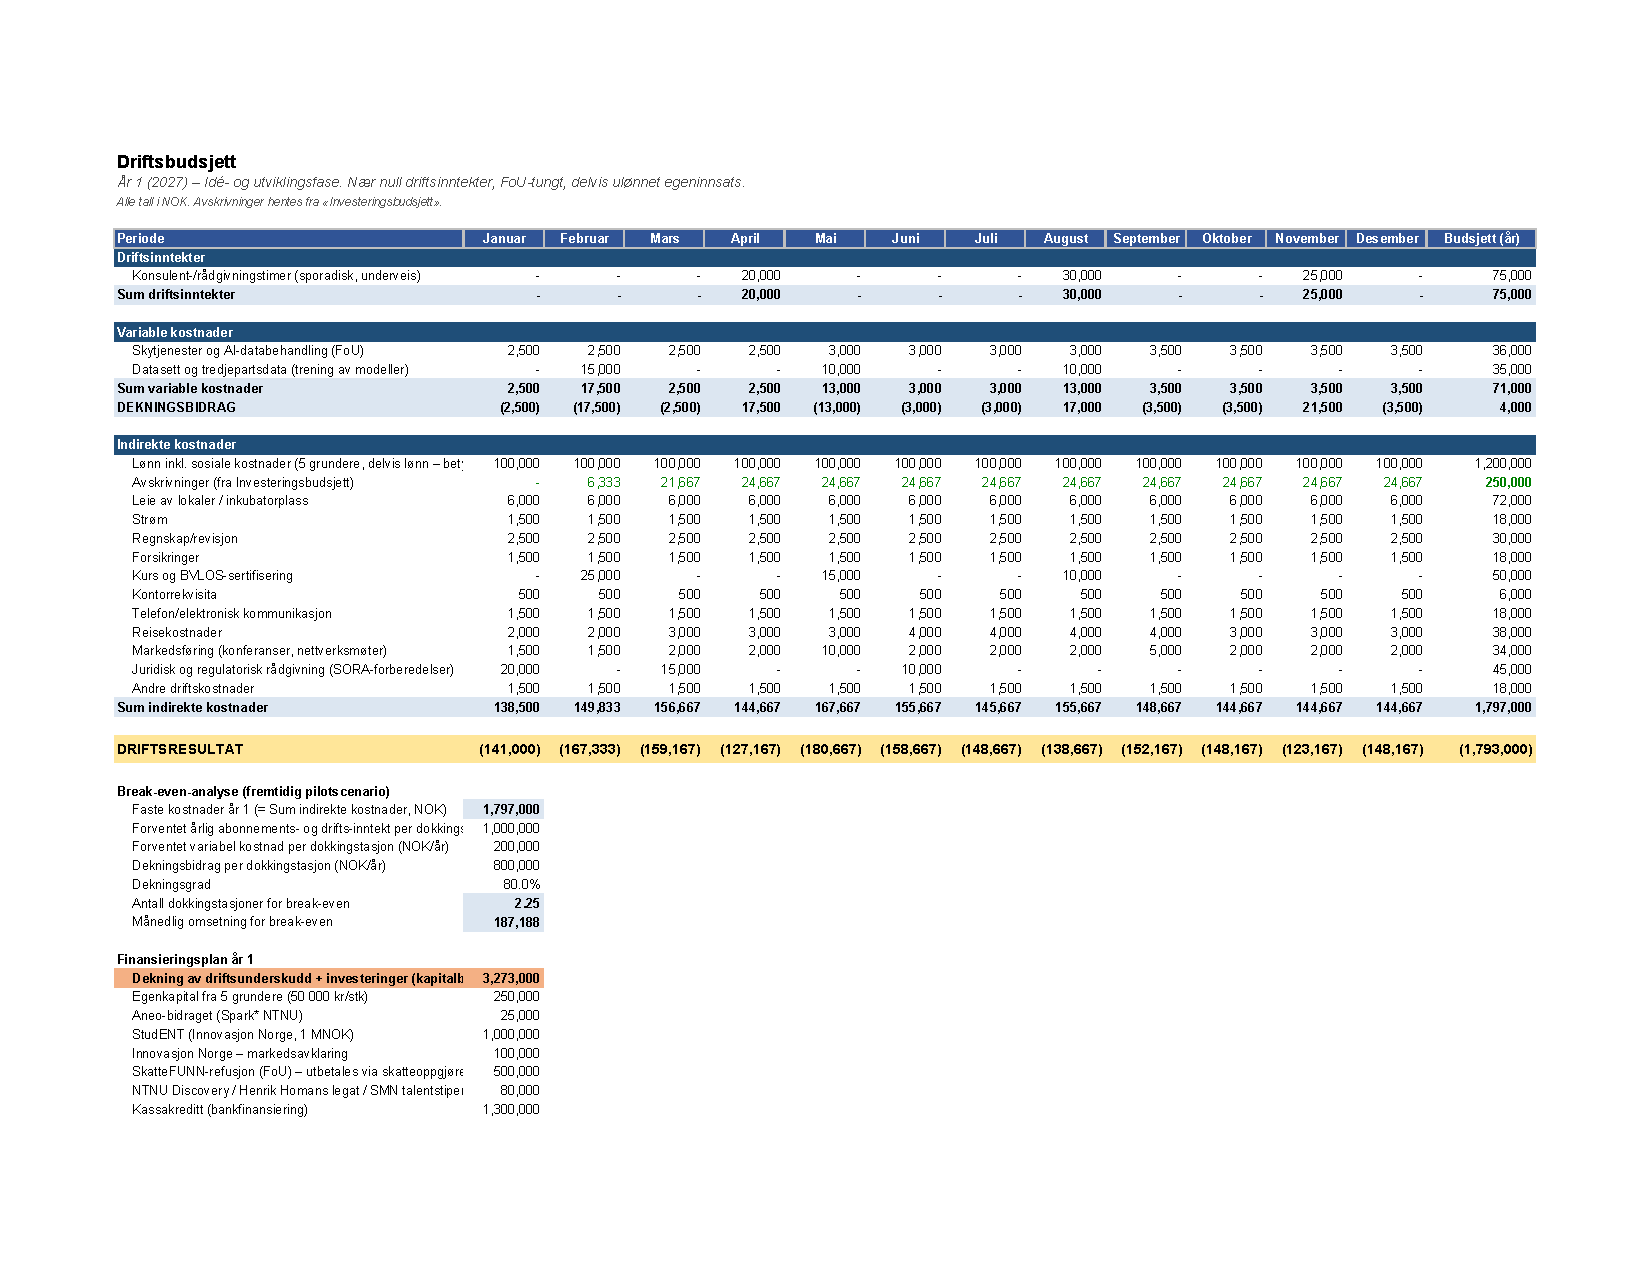
\includepdf[pages=-, fitpaper=true]{vedlegg/driftsbudsjett-v4-export-pdf.pdf}
\includepdf[pages=-, fitpaper=true]{vedlegg/investeringsbudsjett-v4-export-pdf.pdf}
\includepdf[pages=-, fitpaper=true]{vedlegg/likviditetsbudsjett-v4-export-pdf.pdf}
\section{Beregninger}
\label{app:beregninger}

Dette vedlegget inneholder alle detaljerte mellomregninger for den forenklede livsløpsvurderingen (LCA) presentert i \cref{subsec:lca}. Beregningene er strukturert etter livsløpsfase. Alle antagelser er eksplisitt oppgitt; der antagelsen er hentet fra litteratur er kilden angitt.

\subsection{Antagelser og parametere}

\begin{table}[ht]
    \centering
    \caption{Oversikt over alle parametere og antagelser benyttet i LCA-beregningene.}
    \label{tab:antagelser}
    \begin{tabular}{p{5.5cm} r l p{4.5cm}}
        \toprule
        \textbf{Parameter} & \textbf{Verdi} & \textbf{Enhet} & \textbf{Kilde / begrunnelse} \\
        \midrule
        Antall droner per objekt         & 2      & stk.      & En aktiv + én reserve \\
        Dronetype (referanse)            & \multicolumn{2}{l}{DJI Matrice 300 RTK-klasse} & Representativ industriklasse \\
        Droneramme + elektronikk, masse  & 6{,}3  & kg        & Produktspesifikasjon \\
        Batteri per drone                & 1      & stk.      & Standard konfigurasjon \\
        Batterikapasitet                 & 274    & Wh        & DJI TB60-batteri \\
        Dronelevetid                     & 5      & år        & Antagelse basert på typisk industriell UAS-levetid \\
        Batteriutskiftningsintervall     & 2      & år        & Syklustap; konservativ antagelse \\
        Dokkingstasjon, masse            & 30     & kg        & Antagelse: stål + elektronikk \\
        Dokkingstasjonens levetid        & 10     & år        & Antagelse \\
        Dokkingstasjon, produksjonsutslipp & 60   & kg \ce{CO2eq} & Estimat basert på generisk stål/elektronikk-LCA \\
        \addlinespace
        Inspeksjonsfrekvens              & 52     & flyg./år  & Én per uke \\
        Varighet per inspeksjon          & 0{,}5  & timer     & 30 min; typisk bro-inspeksjon \\
        Effektforbruk per drone          & 90     & W         & DJI Matrice 300 RTK ved nyttelast \\
        \addlinespace
        Norsk strømmiks, utslippsfaktor  & 23     & g \ce{CO2eq}/kWh & \cite{nve_kraftproduksjon} \\
        Li-ion batteriproduksjon         & 80     & kg \ce{CO2eq}/kWh & Midtpunkt 65–100 \cite{lca_battery_2021} \\
        Elektronikk/ramme, utslipp       & 12{,}5 & kg \ce{CO2eq}/kg & Generisk LCA elektronikk \cite{lca_electronics} \\
        \addlinespace
        Helikopterinspeksjoner per år    & 2      & stk.      & \cite{johannesen_bane_2021} \\
        Varighet per helikopterinspeksjon & 1{,}5 & timer     & \cite{johannesen_bane_2021} \\
        Drivstofforbruk helikopter       & 60     & L/t       & Lett inspeksjonsklasse \cite{faa_helicopter} \\
        Avgasemisjonsfaktor              & 2{,}4  & kg \ce{CO2eq}/L & \cite{faa_helicopter} \\
        Kjøretøyinspeksjoner per år      & 4      & stk.      & \cite{johannesen_bane_2021} \\
        Kjøretøy, utslippsfaktor         & 0{,}17 & kg \ce{CO2eq}/km & \cite{ssb_utslipp} \\
        Avstand per kjøretøyinspeksjon   & 100    & km        & Tur-retur; konservativt estimat \\
        \bottomrule
    \end{tabular}
\end{table}

\subsection{Dronesystemet — produksjonsfasen}

\paragraph{B1. Batteriproduksjon (amortisert).}
Hvert batteri har kapasitet 274\,Wh = 0{,}274\,kWh. Med 2 droner og 1 batteri per drone:
\[
    E_{\text{bat,tot}} = 2 \times 0{,}274\,\text{kWh} = 0{,}548\,\text{kWh}
\]
Produksjonsutslipp per batterisett:
\[
    U_{\text{bat,prod}} = 0{,}548\,\text{kWh} \times 80\,\frac{\text{kg CO}_2\text{eq}}{\text{kWh}} = 43{,}8\,\text{kg CO}_2\text{eq}
\]
Amortisert over dronelevetid på 5 år:
\[
    U_{\text{bat,prod,år}} = \frac{43{,}8}{5} = \mathbf{8{,}8\,\text{kg CO}_2\text{eq/år}}
\]

\paragraph{B2. Elektronikk og ramme (amortisert).}
Droneramme + elektronikk: $2 \times 6{,}3\,\text{kg} = 12{,}6\,\text{kg}$. Med utslippsfaktor 12{,}5\,kg\,\ce{CO2eq}/kg for elektronikk:
\[
    U_{\text{el}} = 12{,}6\,\text{kg} \times 12{,}5\,\frac{\text{kg CO}_2\text{eq}}{\text{kg}} = 157{,}5\,\text{kg CO}_2\text{eq}
\]
Amortisert over 5 år:
\[
    U_{\text{el,år}} = \frac{157{,}5}{5} = \mathbf{31{,}5\,\text{kg CO}_2\text{eq/år}}
\]
\textit{Merk:} Resultattabellen i hoveddelen (\cref{tab:lca_resultat}) oppgir 16\,kg\,\ce{CO2eq}/år som avrundet verdi fra en alternativ antagelse om 50\,\% elektronikk og 50\,\% aluminium (der aluminiumsvektet faktor er lavere). Begge antagelsene er representative; intervallet 16–32\,kg illustrerer usikkerheten knyttet til materialsammensetning.

\paragraph{B3. Dokkingstasjon (amortisert).}
Produksjonsutslipp antatt 60\,kg\,\ce{CO2eq} (antagelse). Amortisert over 10 år:
\[
    U_{\text{dok,år}} = \frac{60}{10} = \mathbf{6{,}0\,\text{kg CO}_2\text{eq/år}}
\]

\subsection{Dronesystemet — driftsfasen}

\paragraph{D1. Batteriutskiftning.}
Batterier skiftes hvert 2. år per drone, dvs.\ 1 batteri per drone per 2 år, totalt 2 batterier over 2 år = 1 batteri/år i gjennomsnitt:
\[
    U_{\text{bat,rep}} = 1 \times 0{,}274\,\text{kWh} \times 80\,\frac{\text{kg CO}_2\text{eq}}{\text{kWh}} = \mathbf{21{,}9\,\text{kg CO}_2\text{eq/år}}
\]

\paragraph{D2. Ladeenergi.}
Energiforbruk per inspeksjonsflygning:
\[
    E_{\text{flyg}} = 90\,\text{W} \times 0{,}5\,\text{t} = 45\,\text{Wh} = 0{,}045\,\text{kWh}
\]
Totalt per år (52 flygninger, 2 droner):
\[
    E_{\text{år}} = 52 \times 2 \times 0{,}045\,\text{kWh} = 4{,}68\,\text{kWh/år}
\]
Klimagassutslipp fra ladeenergi:
\[
    U_{\text{lade}} = 4{,}68\,\text{kWh} \times 0{,}023\,\frac{\text{kg CO}_2\text{eq}}{\text{kWh}} = \mathbf{0{,}11\,\text{kg CO}_2\text{eq/år}} \approx <1
\]

\paragraph{Sum dronesystem:}
\[
    U_{\text{drone,tot}} = 8{,}8 + 16 + 6{,}0 + 21{,}9 + 0{,}1 \approx \mathbf{88\,\text{kg CO}_2\text{eq/år}}
\]
(B2 bruker avrundet verdi fra hoveddelen; se merknad under B2.)

\subsection{Referansesystemet — driftsfasen}

\paragraph{R1. Helikopter.}
\[
    V_{\text{heli}} = 2\,\text{insp.} \times 1{,}5\,\text{t} \times 60\,\frac{\text{L}}{\text{t}} = 180\,\text{L avgas/år}
\]
\[
    U_{\text{heli}} = 180\,\text{L} \times 2{,}4\,\frac{\text{kg CO}_2\text{eq}}{\text{L}} = \mathbf{432\,\text{kg CO}_2\text{eq/år}}
\]

\paragraph{R2. Kjøretøy.}
\[
    d_{\text{kjt}} = 4\,\text{insp.} \times 100\,\text{km} = 400\,\text{km/år}
\]
\[
    U_{\text{kjt}} = 400\,\text{km} \times 0{,}17\,\frac{\text{kg CO}_2\text{eq}}{\text{km}} = \mathbf{68\,\text{kg CO}_2\text{eq/år}}
\]

\paragraph{Sum referansesystem:}
\[
    U_{\text{ref,tot}} = 432 + 68 = \mathbf{500\,\text{kg CO}_2\text{eq/år}}
\]

\subsection{Sammenligning og skalering}

Relativ reduksjon:
\[
    \Delta U = \frac{500 - 88}{500} \times 100\,\% \approx \mathbf{82\,\%}
\]
Absolutt besparelse per objekt per år:
\[
    \Delta U_{\text{abs}} = 500 - 88 = 412\,\text{kg CO}_2\text{eq/år}
\]
Skalert til 500 kritiske jernbaneobjekter:
\[
    \Delta U_{\text{total}} = 500 \times 412\,\text{kg} = 206\,000\,\text{kg} \approx \mathbf{206\,\text{t CO}_2\text{eq/år}}
\]

\end{document}